\documentclass[11pt]{beamer}
%\usetheme{Warsaw}
% for themes, etc.
\mode<presentation>
%\usetheme{Warsaw}
%\usecolortheme{dolphin}
%{\usetheme{Singapore}}
%{ \usetheme{lined} }
\usetheme{CambridgeUS}
\usepackage{amsmath,amssymb,amsfonts,booktabs} 
\usepackage{epic}
\usepackage{mathpazo}
\usepackage{subfigure}
\usepackage{hyperref}
%%%%%%%%%%製造漸層效果背景
\def\softness{0.9}
\definecolor{softrb}{rgb}{1,\softness,1}
\colorlet{darkred}{red!80!black}
\beamertemplateshadingbackground{softrb}{blue!2}%{structure!10}
\beamertemplatetransparentcovereddynamic \beamertemplateballitem
\beamertemplatenumberedballsectiontoc
%%%%%%%%%%%%%%%%%%%%%%%%%%%%%
% fonts are up to you
%\usepackage{astats,epsfig}
\usepackage{graphicx,epsfig}
\usepackage{xcolor}
\usepackage{mathrsfs}
\newtheorem{thm}{\bf{Theorem.}}
\renewcommand{\proofname}{\ctxfk \textbf{Proof.}}
\usepackage{hyperref}
% these will be used later in the title page
\title{Music Feature}
\subtitle{Music Genre Classification}
\author{Yi-Hsin Lu}
\date{June 9, 2022}
\begin{document}
%cover titlepage
\begin{frame}
\titlepage
\end{frame}
%outline
\begin{frame}
    \frametitle{Outline}
    \tableofcontents%[pausesections] %[pausesections] 表示一項一項列出
\end{frame}

\section{Introduction}
\begin{frame}{Motivating Question}
\begin{itemize}
    \item Music
\end{itemize}
\end{frame}

\begin{frame}{Focus Problem}
\begin{itemize}
    \item classify the music genre
\end{itemize}
\begin{center}
    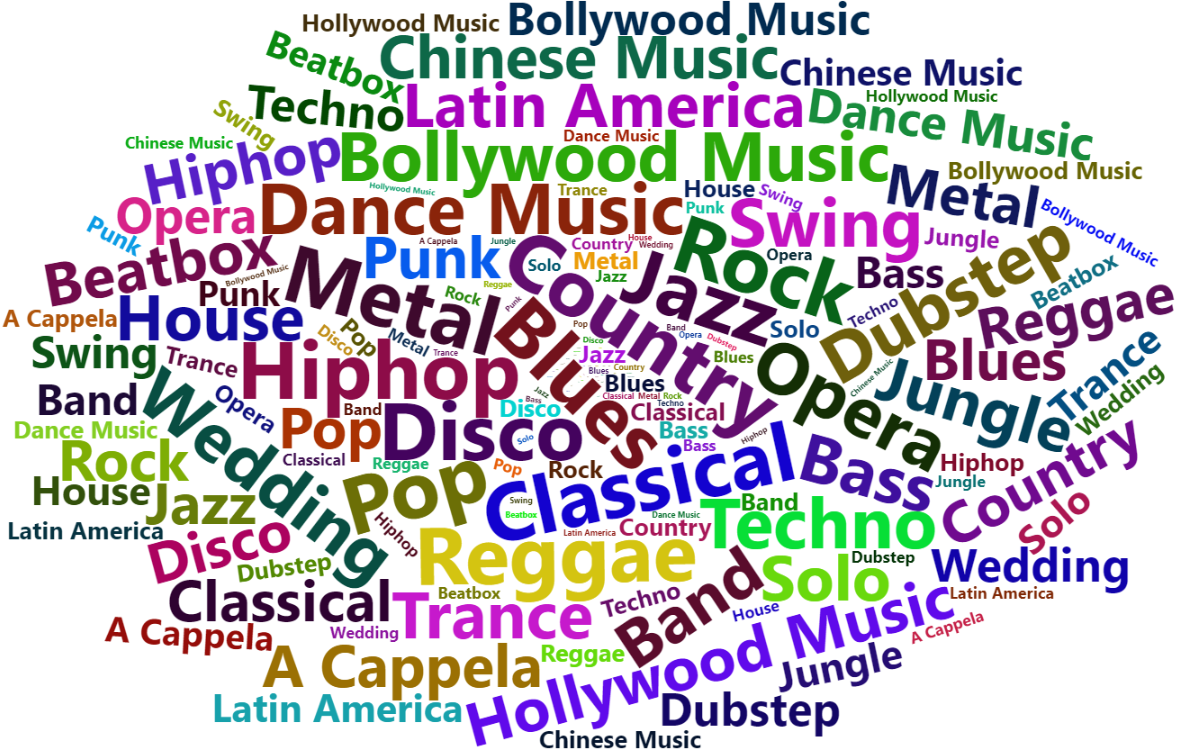
\includegraphics[width=0.8\textwidth]{wordCloud.png}
\end{center}
\end{frame}

\section{Data}
\begin{frame}{Data Set}
\begin{itemize}
    \item \href{https://www.kaggle.com/datasets/insiyeah/musicfeatures}{Kaggle}
    \item 1000 audio files
    \item 28 features
    \item 10 genres
\end{itemize}
\begin{center}
    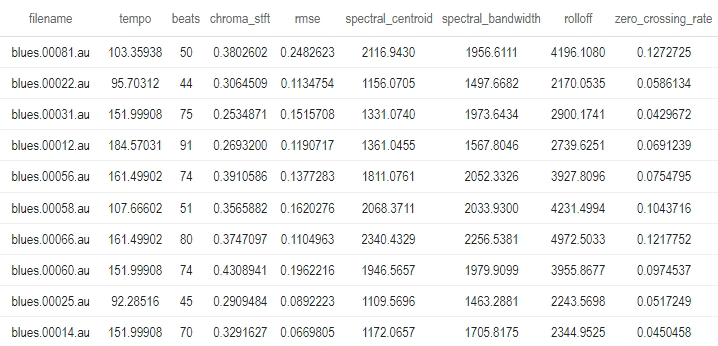
\includegraphics[width=0.8\textwidth]{data.jpg}
\end{center}
\end{frame}

\begin{frame}{Features(28)}
\begin{itemize}
  \item tempo
  \item beats
  \item chroma-stft
  \item rmse
  \item spectral-centroid
  \item spectral-bandwidth
  \item rolloff
  \item zero-crossing-rate
  \item mfcc1-20
\end{itemize}
\end{frame}

\begin{frame}{Genre(10)}
\begin{itemize}
  \item blues
  \item classical
  \item country
  \item disco
  \item hiphop
  \item jazz
  \item metal
  \item pop
  \item reggae
  \item rock
\end{itemize}
\end{frame}

\section{EDA}
\begin{frame}{Correlation Matrix}
\begin{center}
    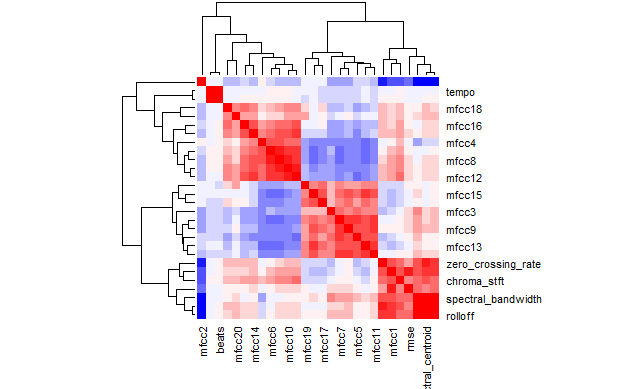
\includegraphics[width=0.8\textwidth]{correlation_matrix.png}
\end{center}
\end{frame}

\begin{frame}{Pair plot}
\begin{center}
    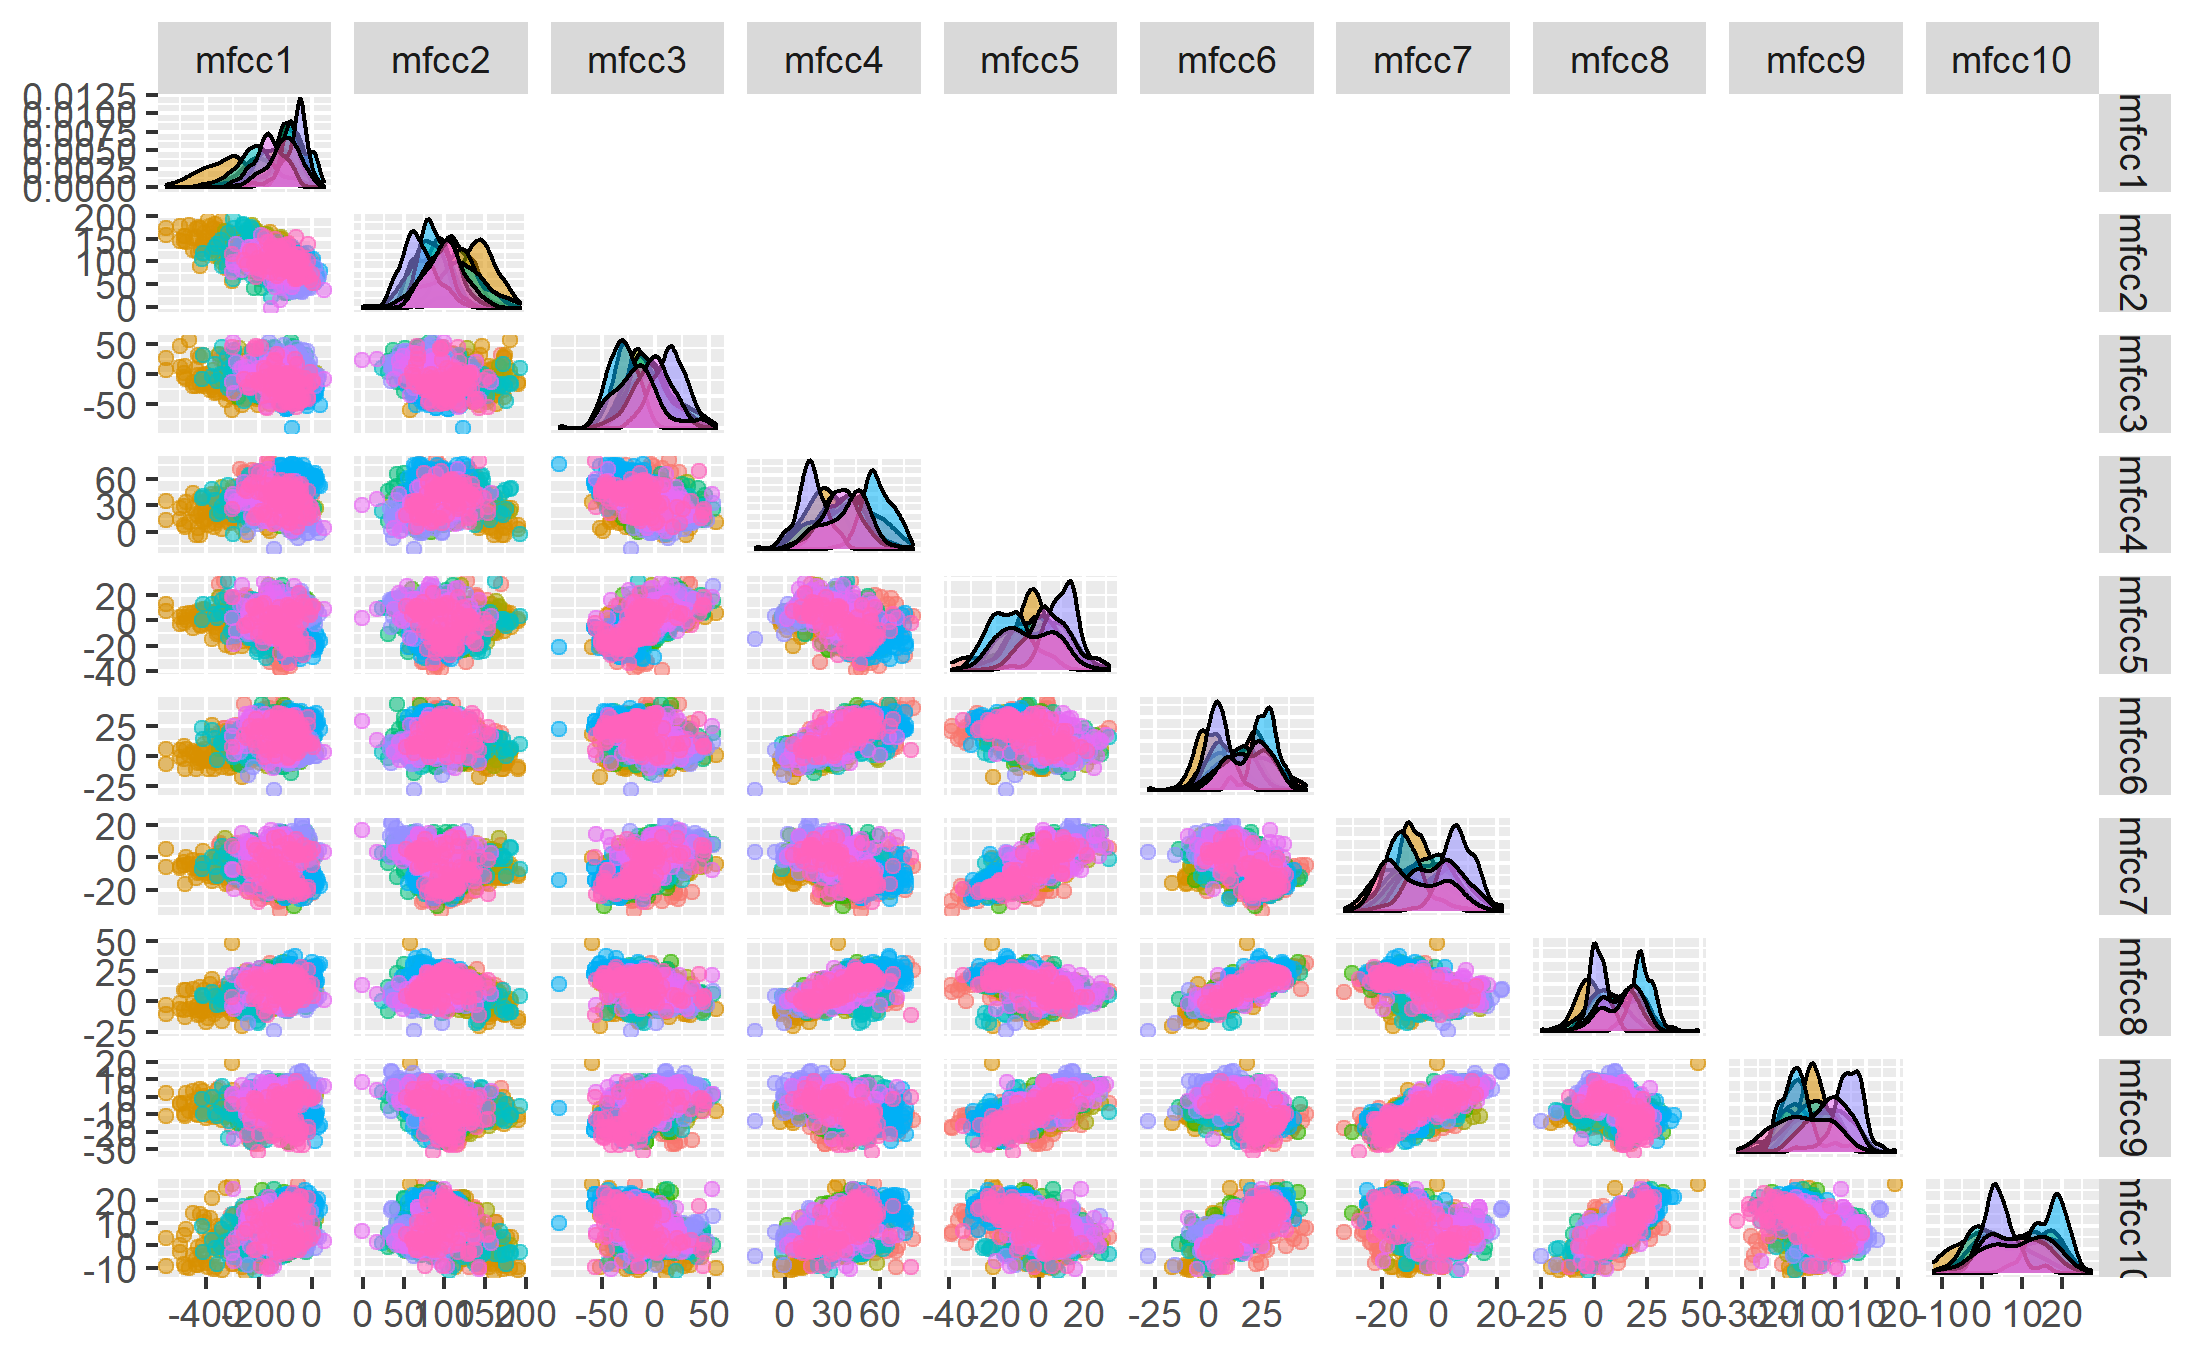
\includegraphics[width=0.8\textwidth]{ggpairs2.png}
\end{center}
\end{frame}
\begin{frame}{Pair plot}
\begin{center}
    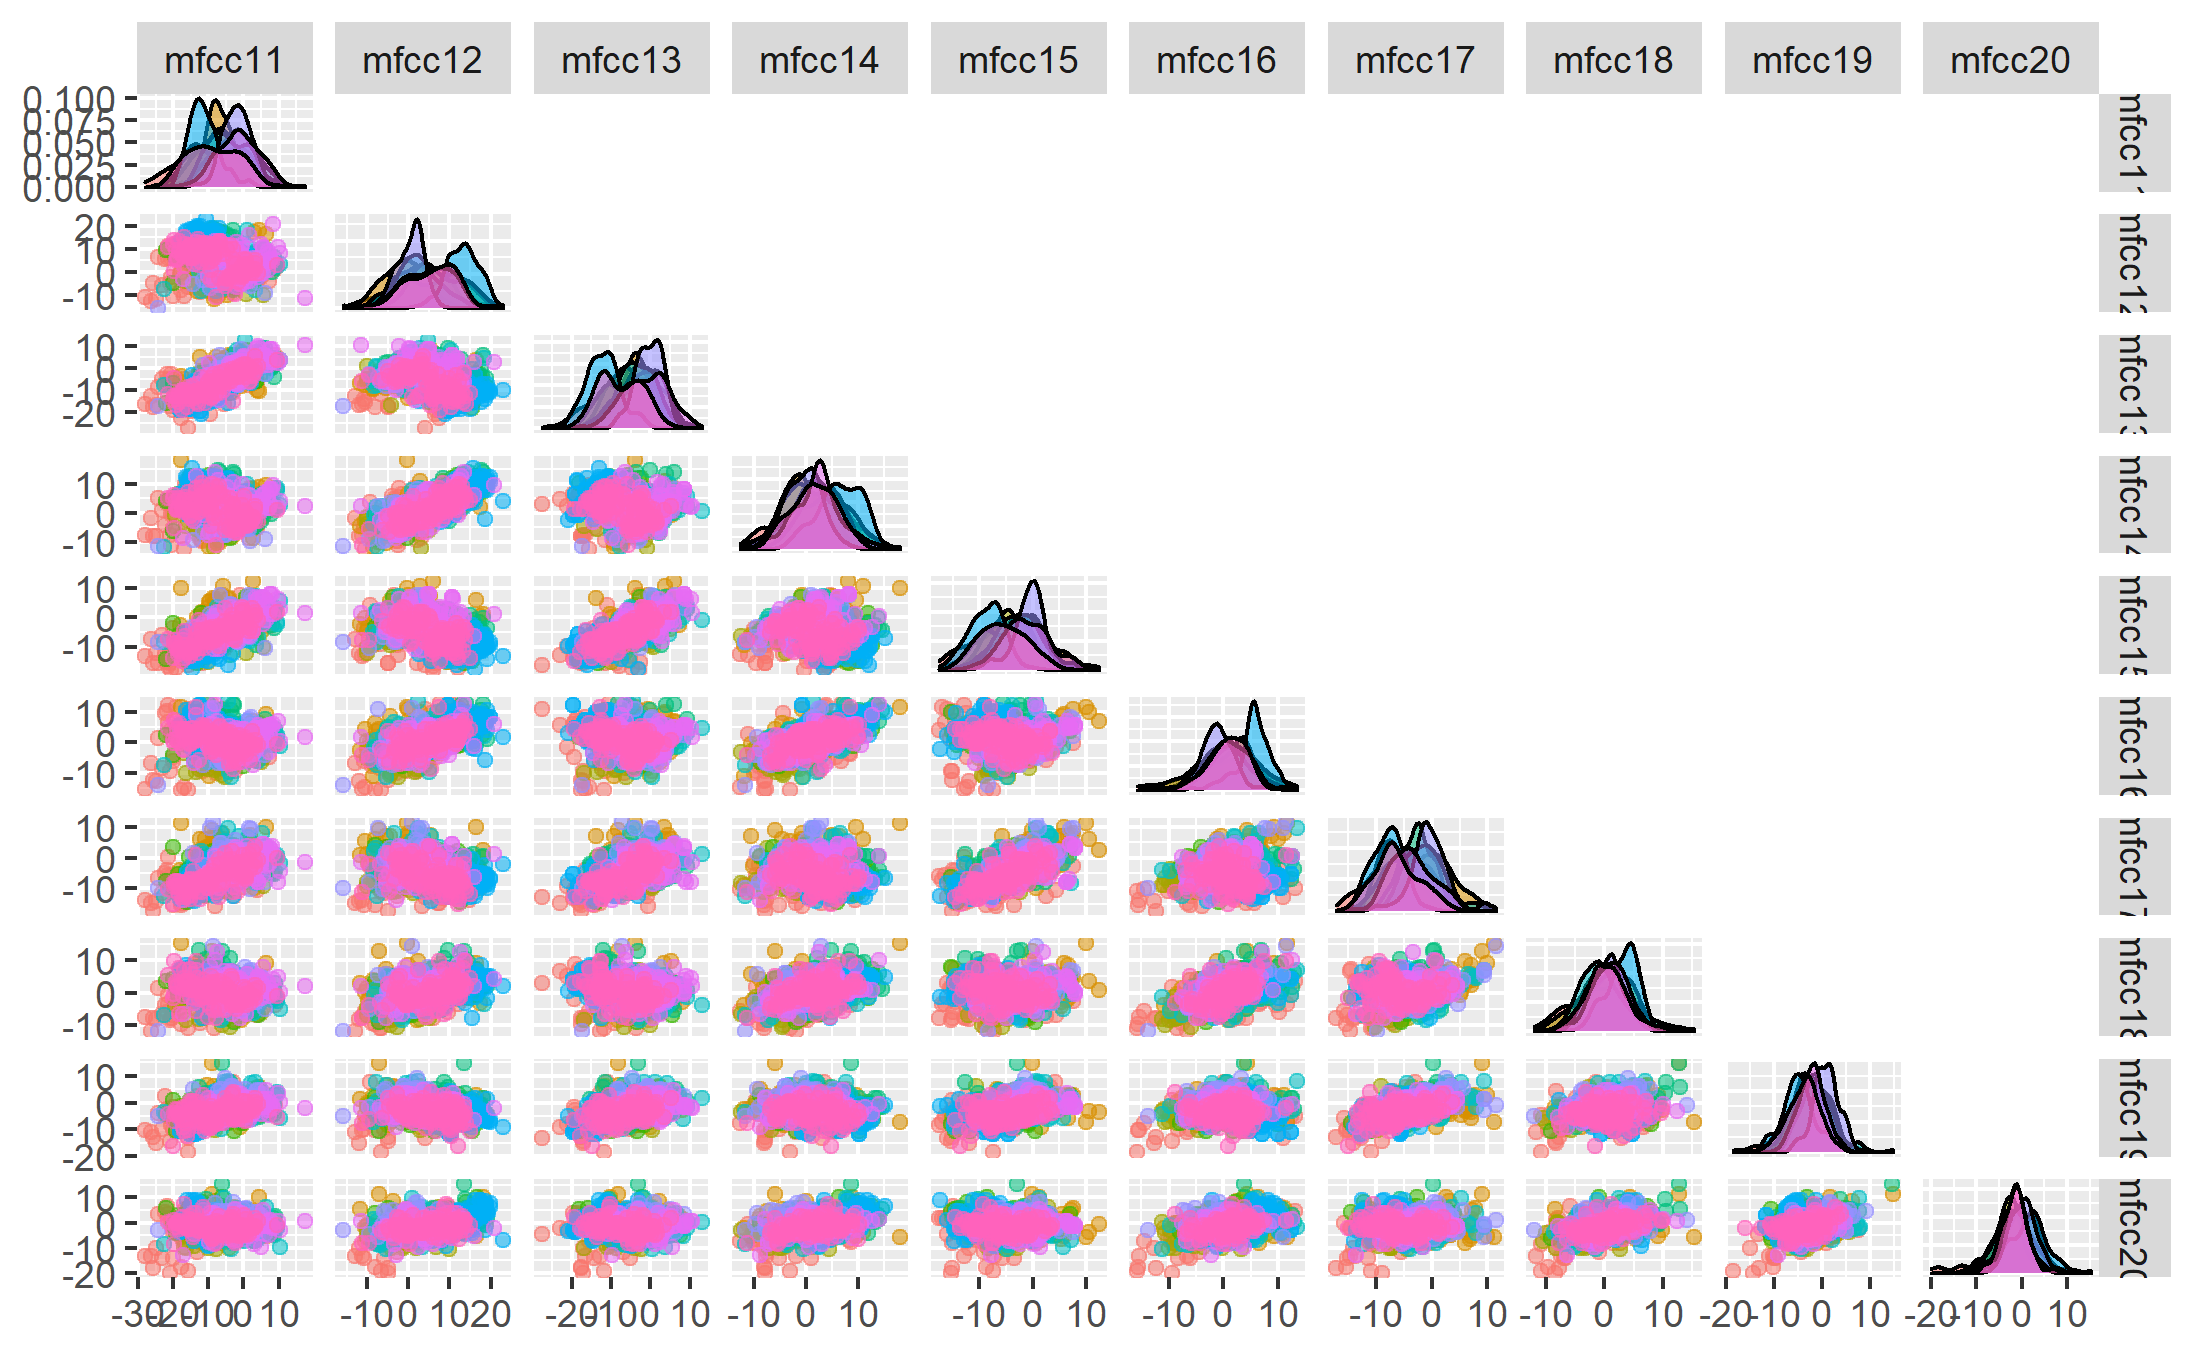
\includegraphics[width=0.8\textwidth]{ggpairs3.png}
\end{center}
\end{frame}
\begin{frame}{Pair plot}
\begin{center}
    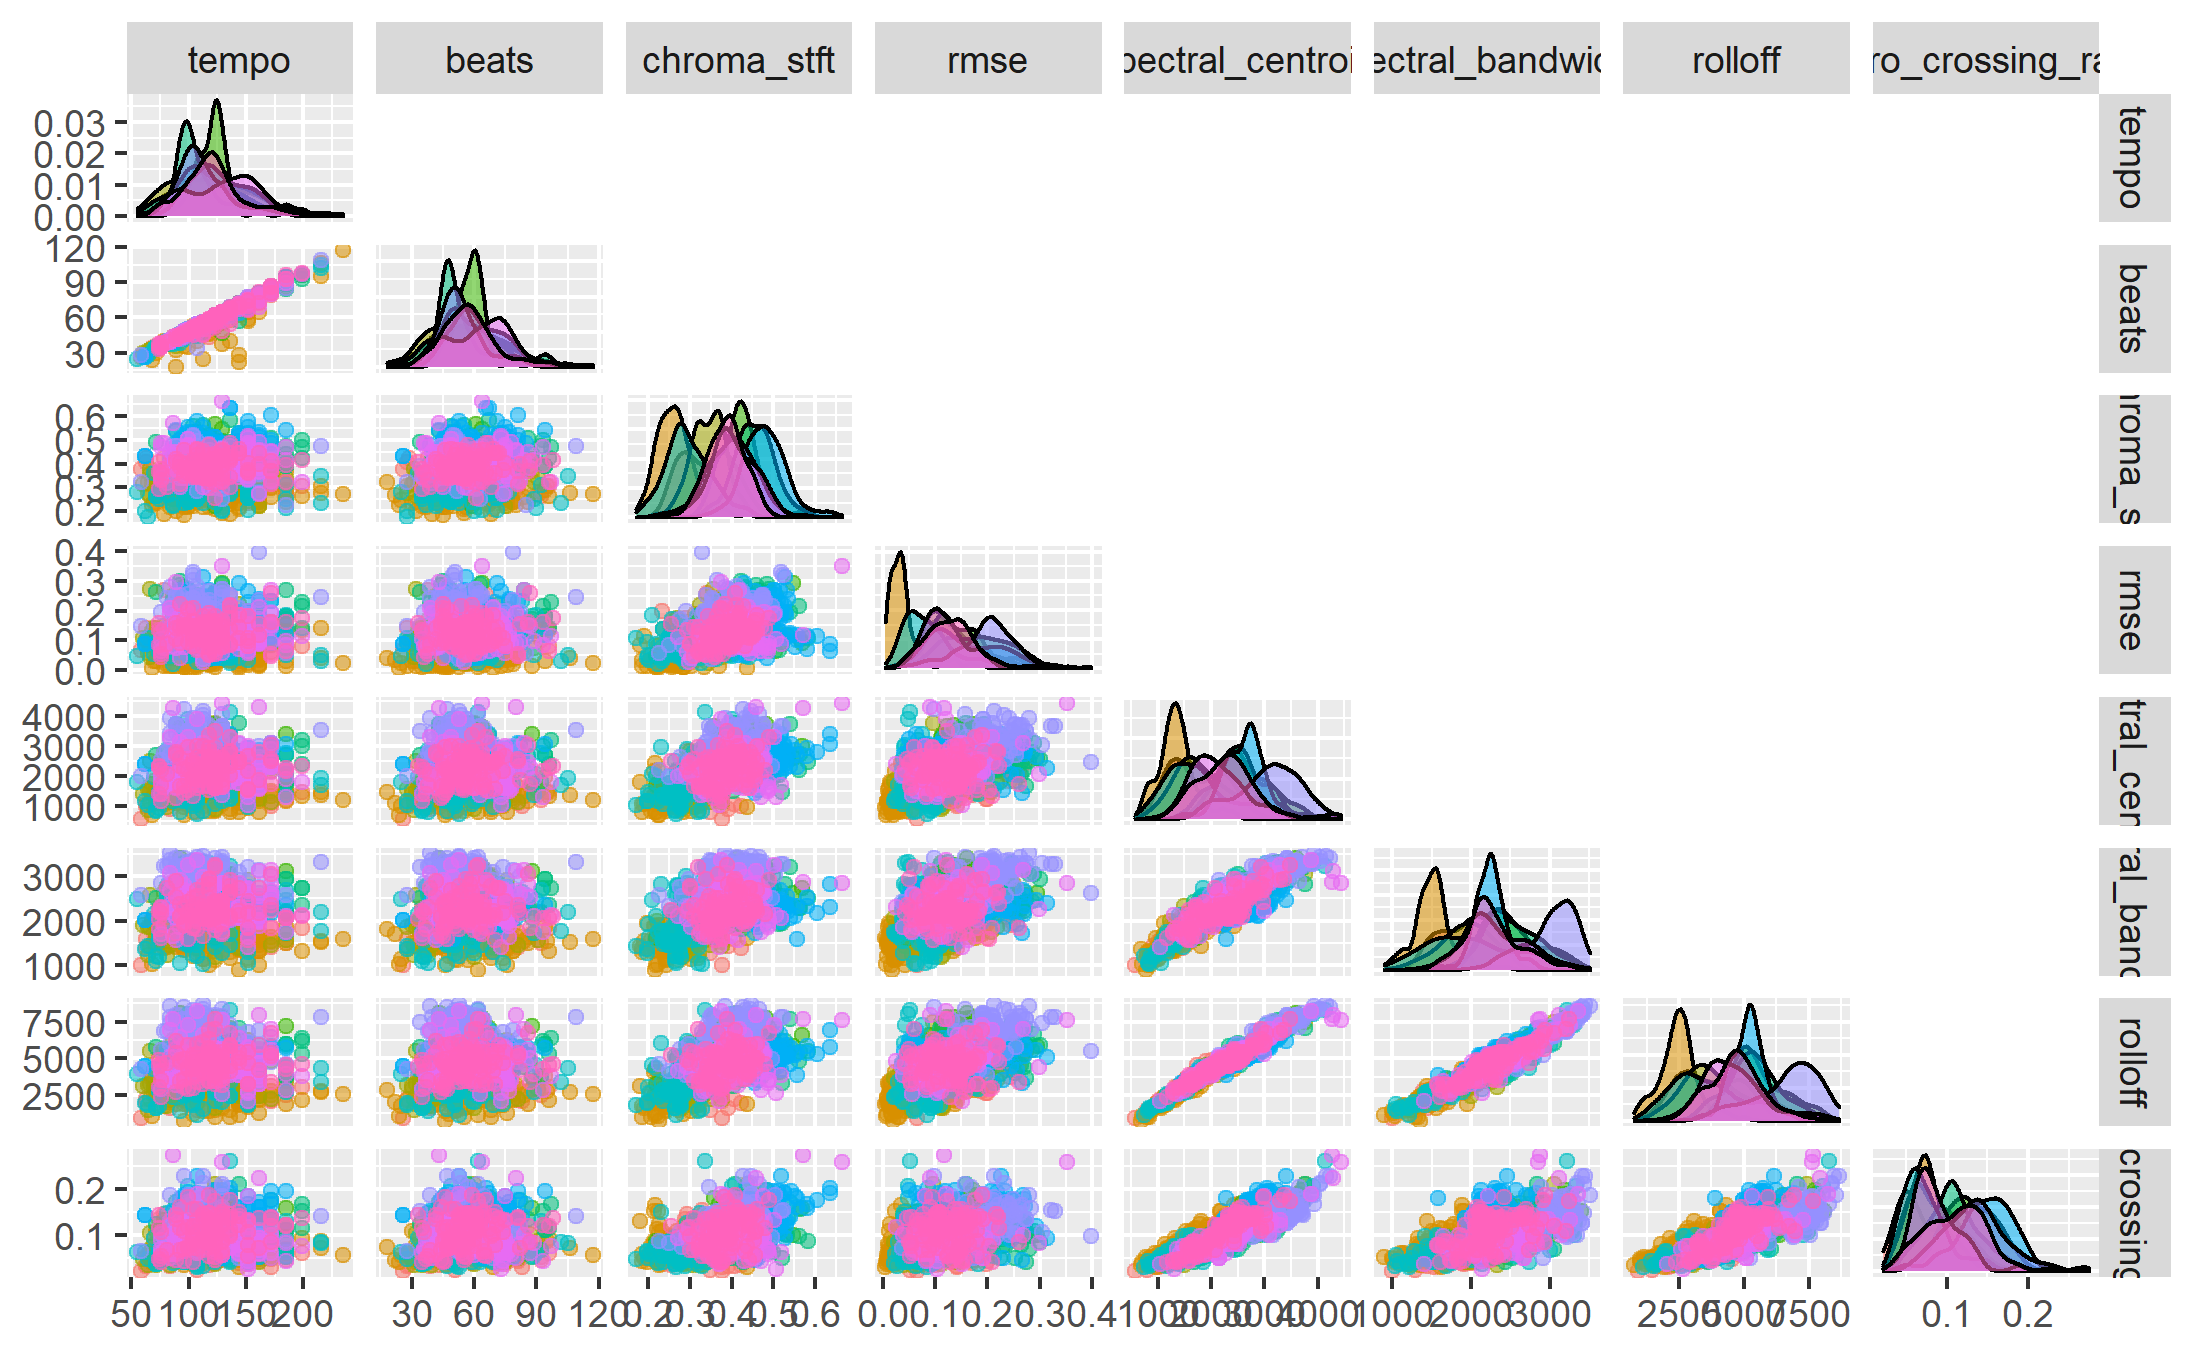
\includegraphics[width=0.8\textwidth]{ggpairs1.png}
\end{center}
\end{frame}

\begin{frame}{PCA(features)}
\begin{center}
    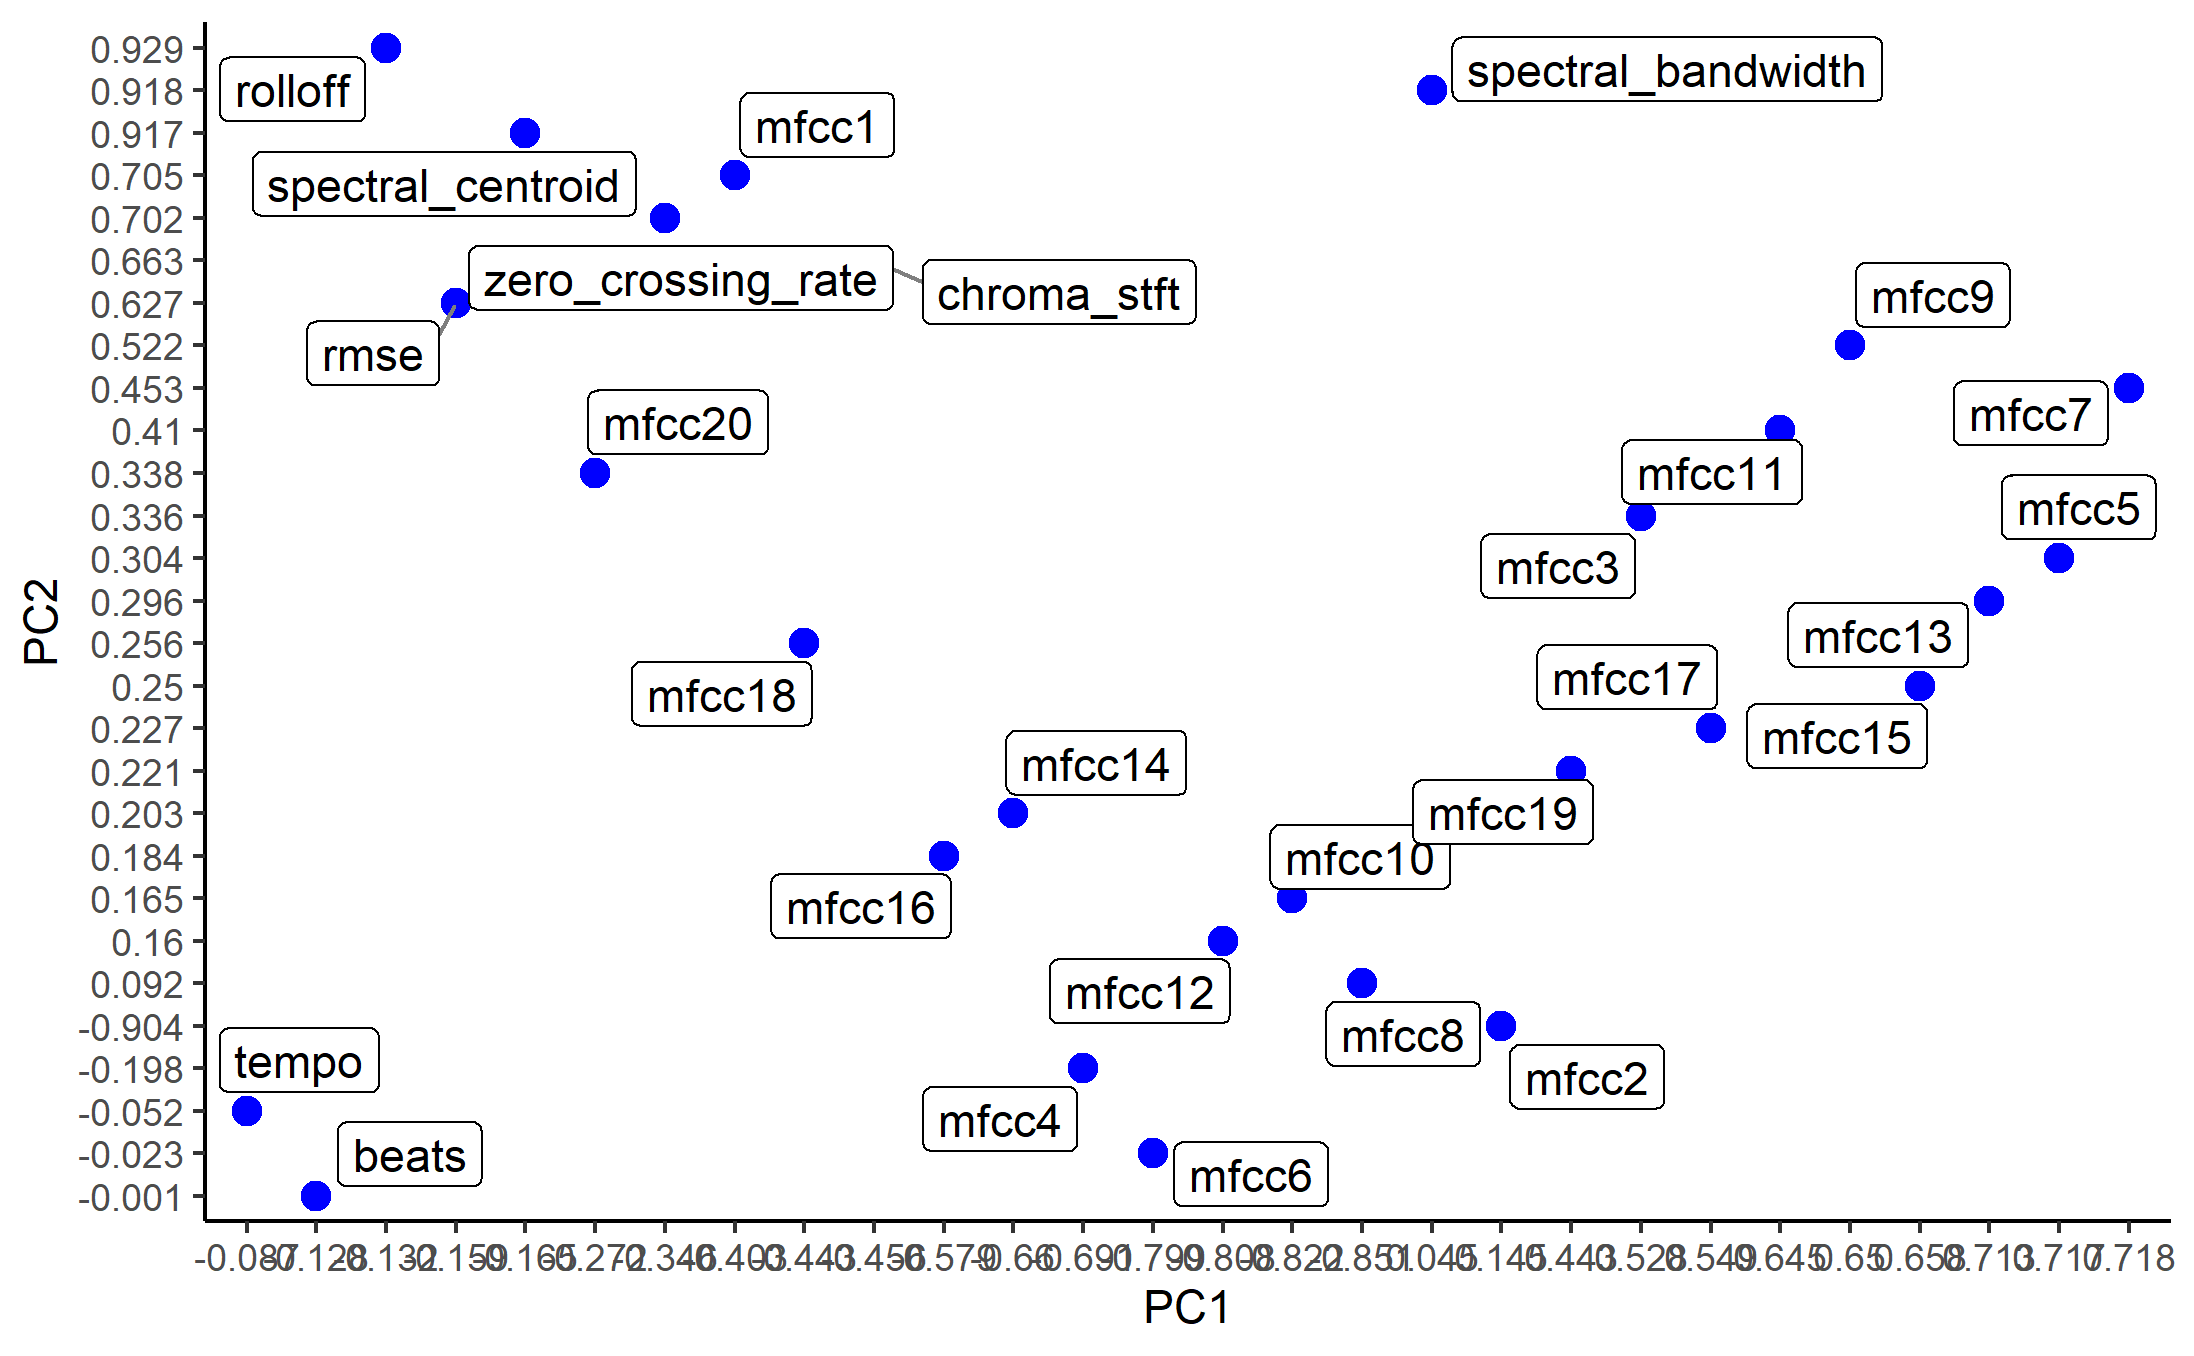
\includegraphics[width=0.8\textwidth]{pca_feat.png}
\end{center}
\end{frame}

\begin{frame}{PCA(audio)}
\begin{center}
    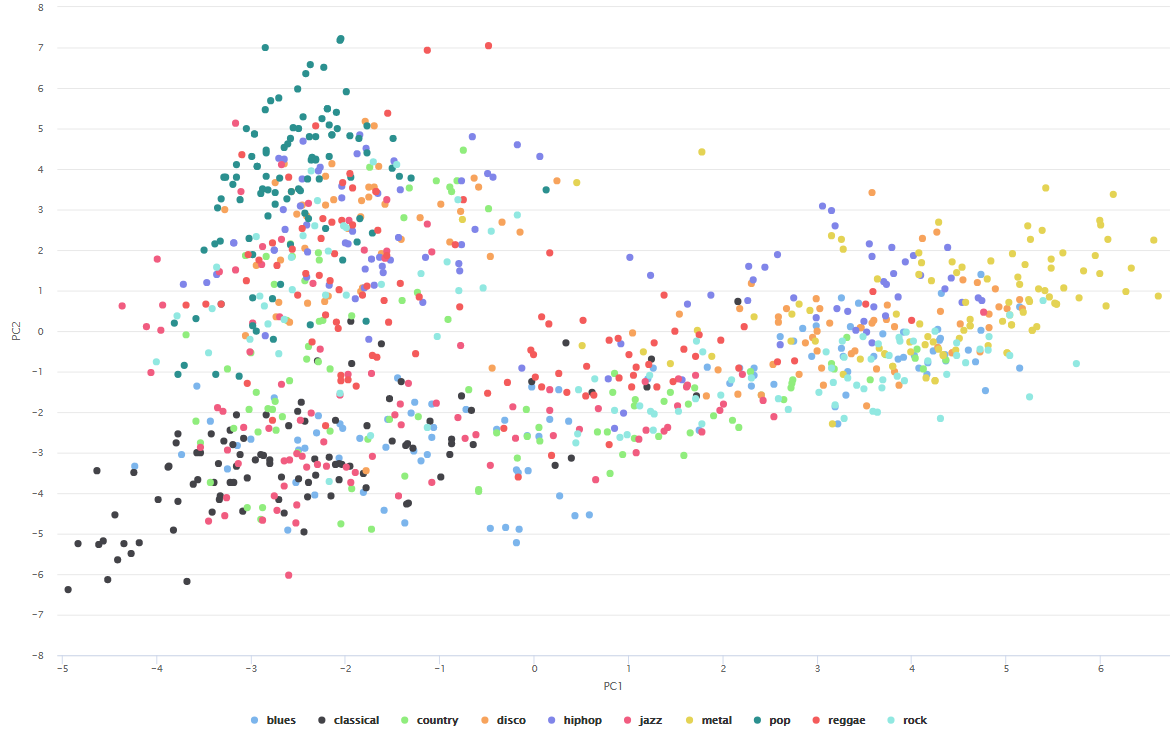
\includegraphics[width=0.8\textwidth]{pca.png}
\end{center}
\end{frame}

\section{Model}

\begin{frame}{Training/Testing Data}
\begin{itemize}
    \item Training: 800
    \item Testing: 200
\end{itemize}
\end{frame}

\begin{frame}{Logistic Regression}
\begin{center}
    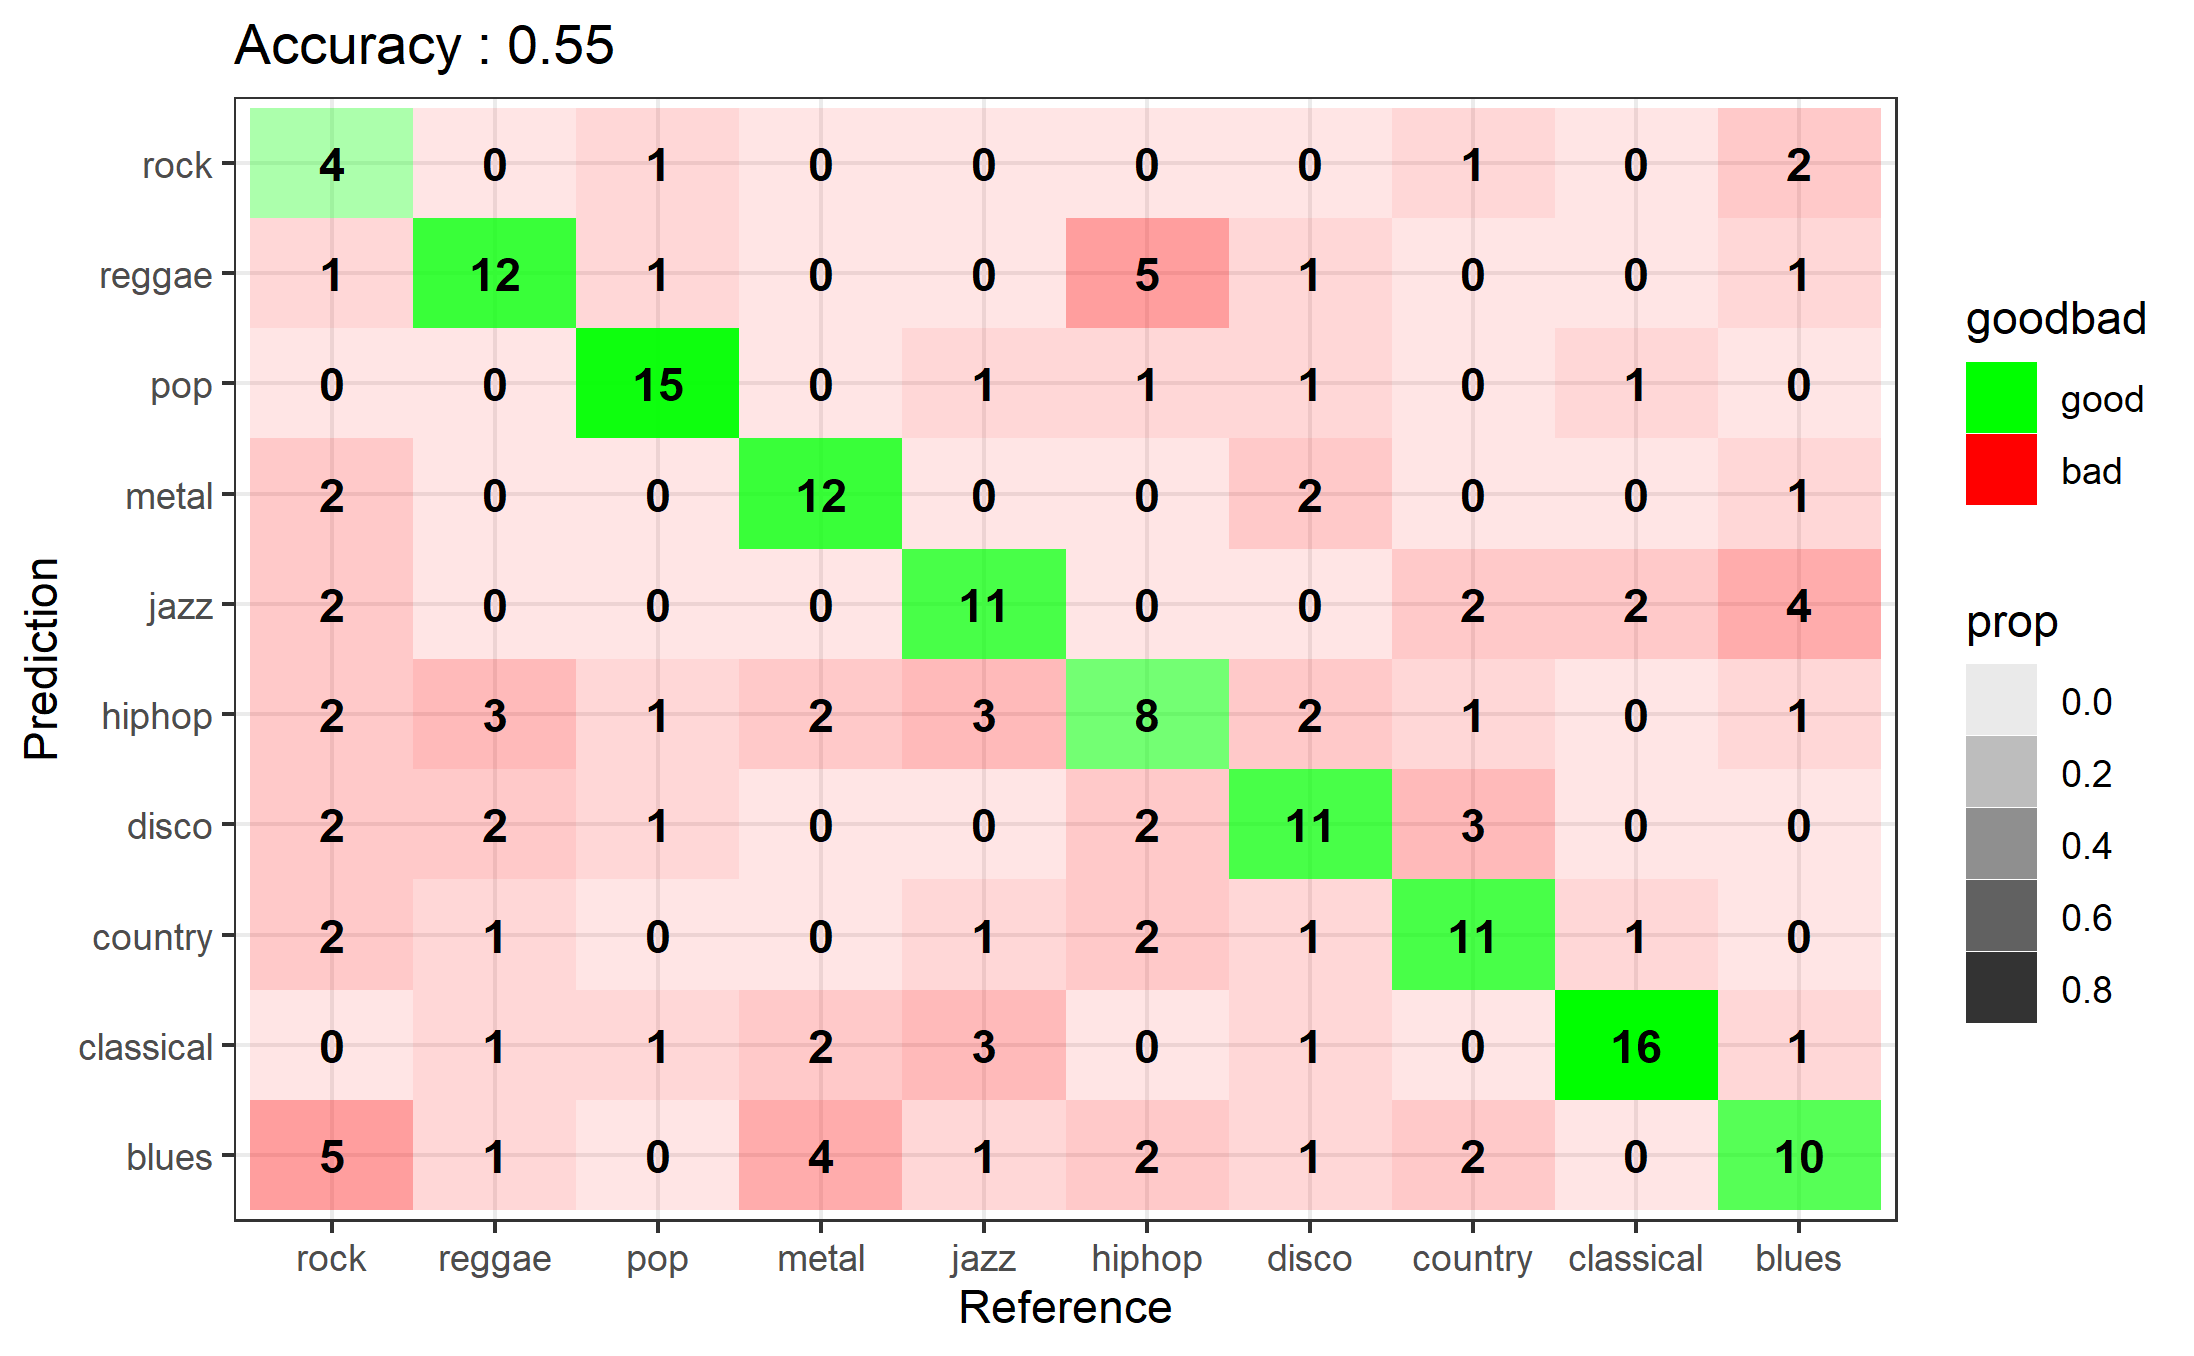
\includegraphics[width=0.8\textwidth]{confusionMatrix_logreg.png}
\end{center}
\end{frame}

\begin{frame}{One-hot encoding}
\begin{itemize}
\end{itemize}
\begin{center}
    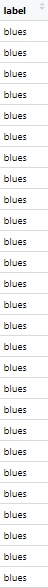
\includegraphics[height=0.5\textwidth]{y.jpg}
    $\Longrightarrow$
    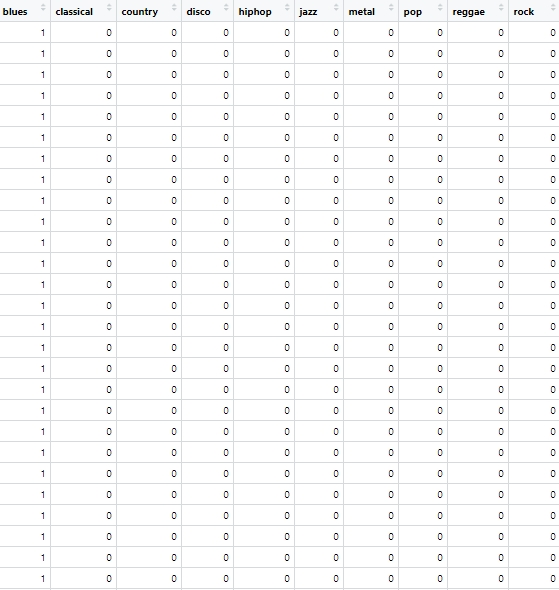
\includegraphics[height=0.5\textwidth]{y_matrix.jpg}
\end{center}
\end{frame}

\begin{frame}{SVM}
\begin{itemize}
    \item Predict for each genre
\end{itemize}
\begin{center}
    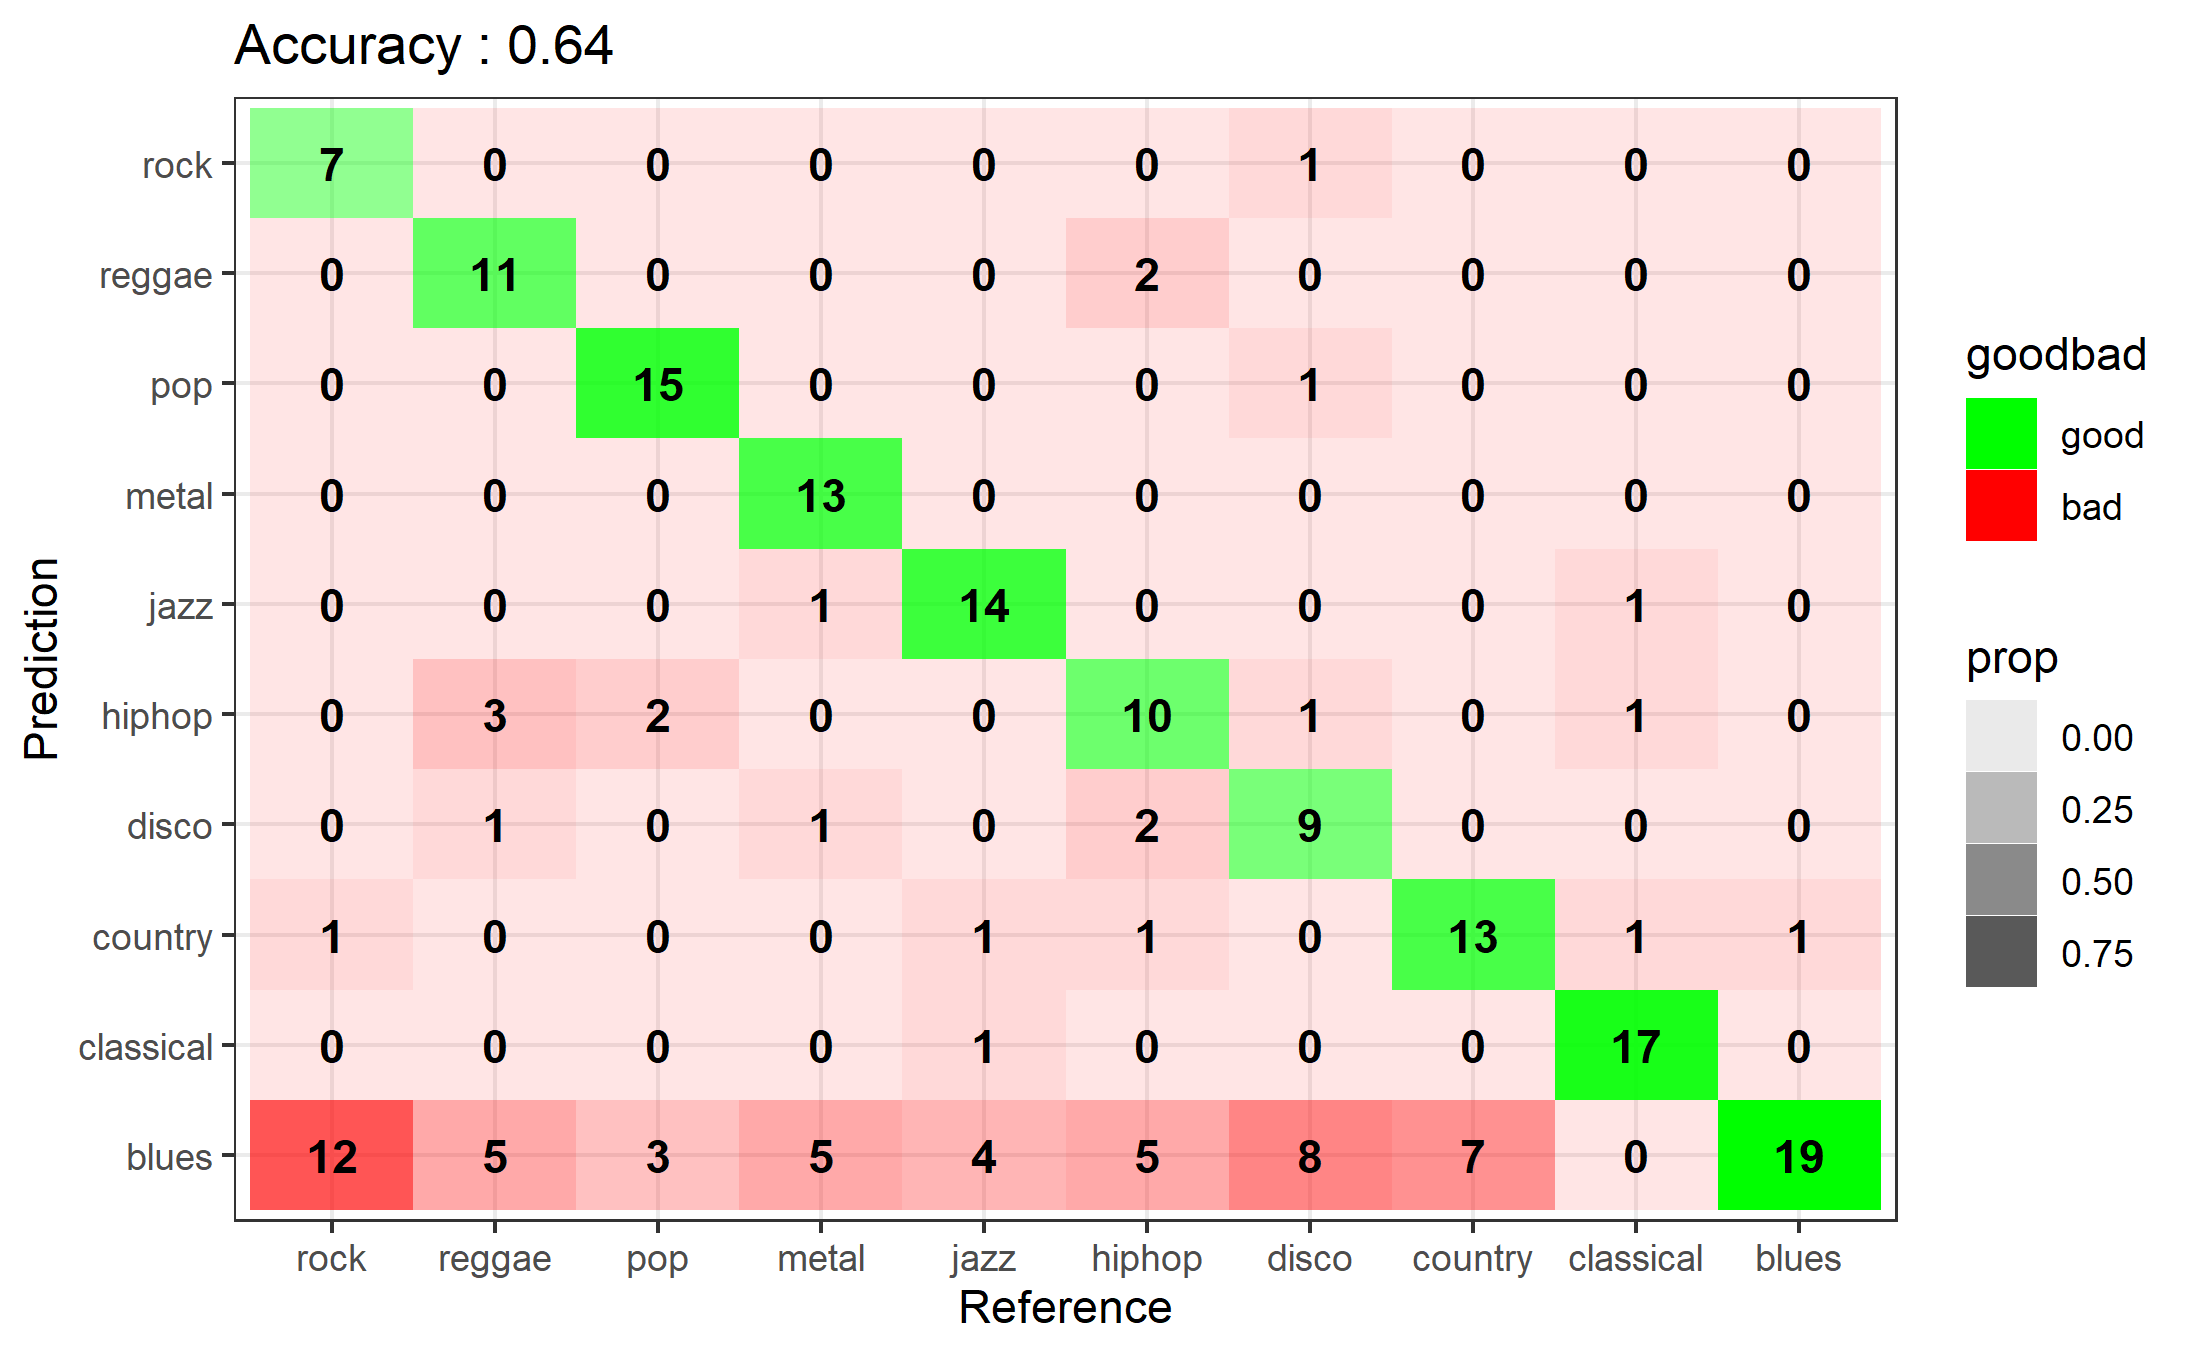
\includegraphics[width=0.8\textwidth]{confusionMatrix_ohencoding_std.png}
\end{center}
\end{frame}

\begin{frame}{SVM}
\begin{center}
    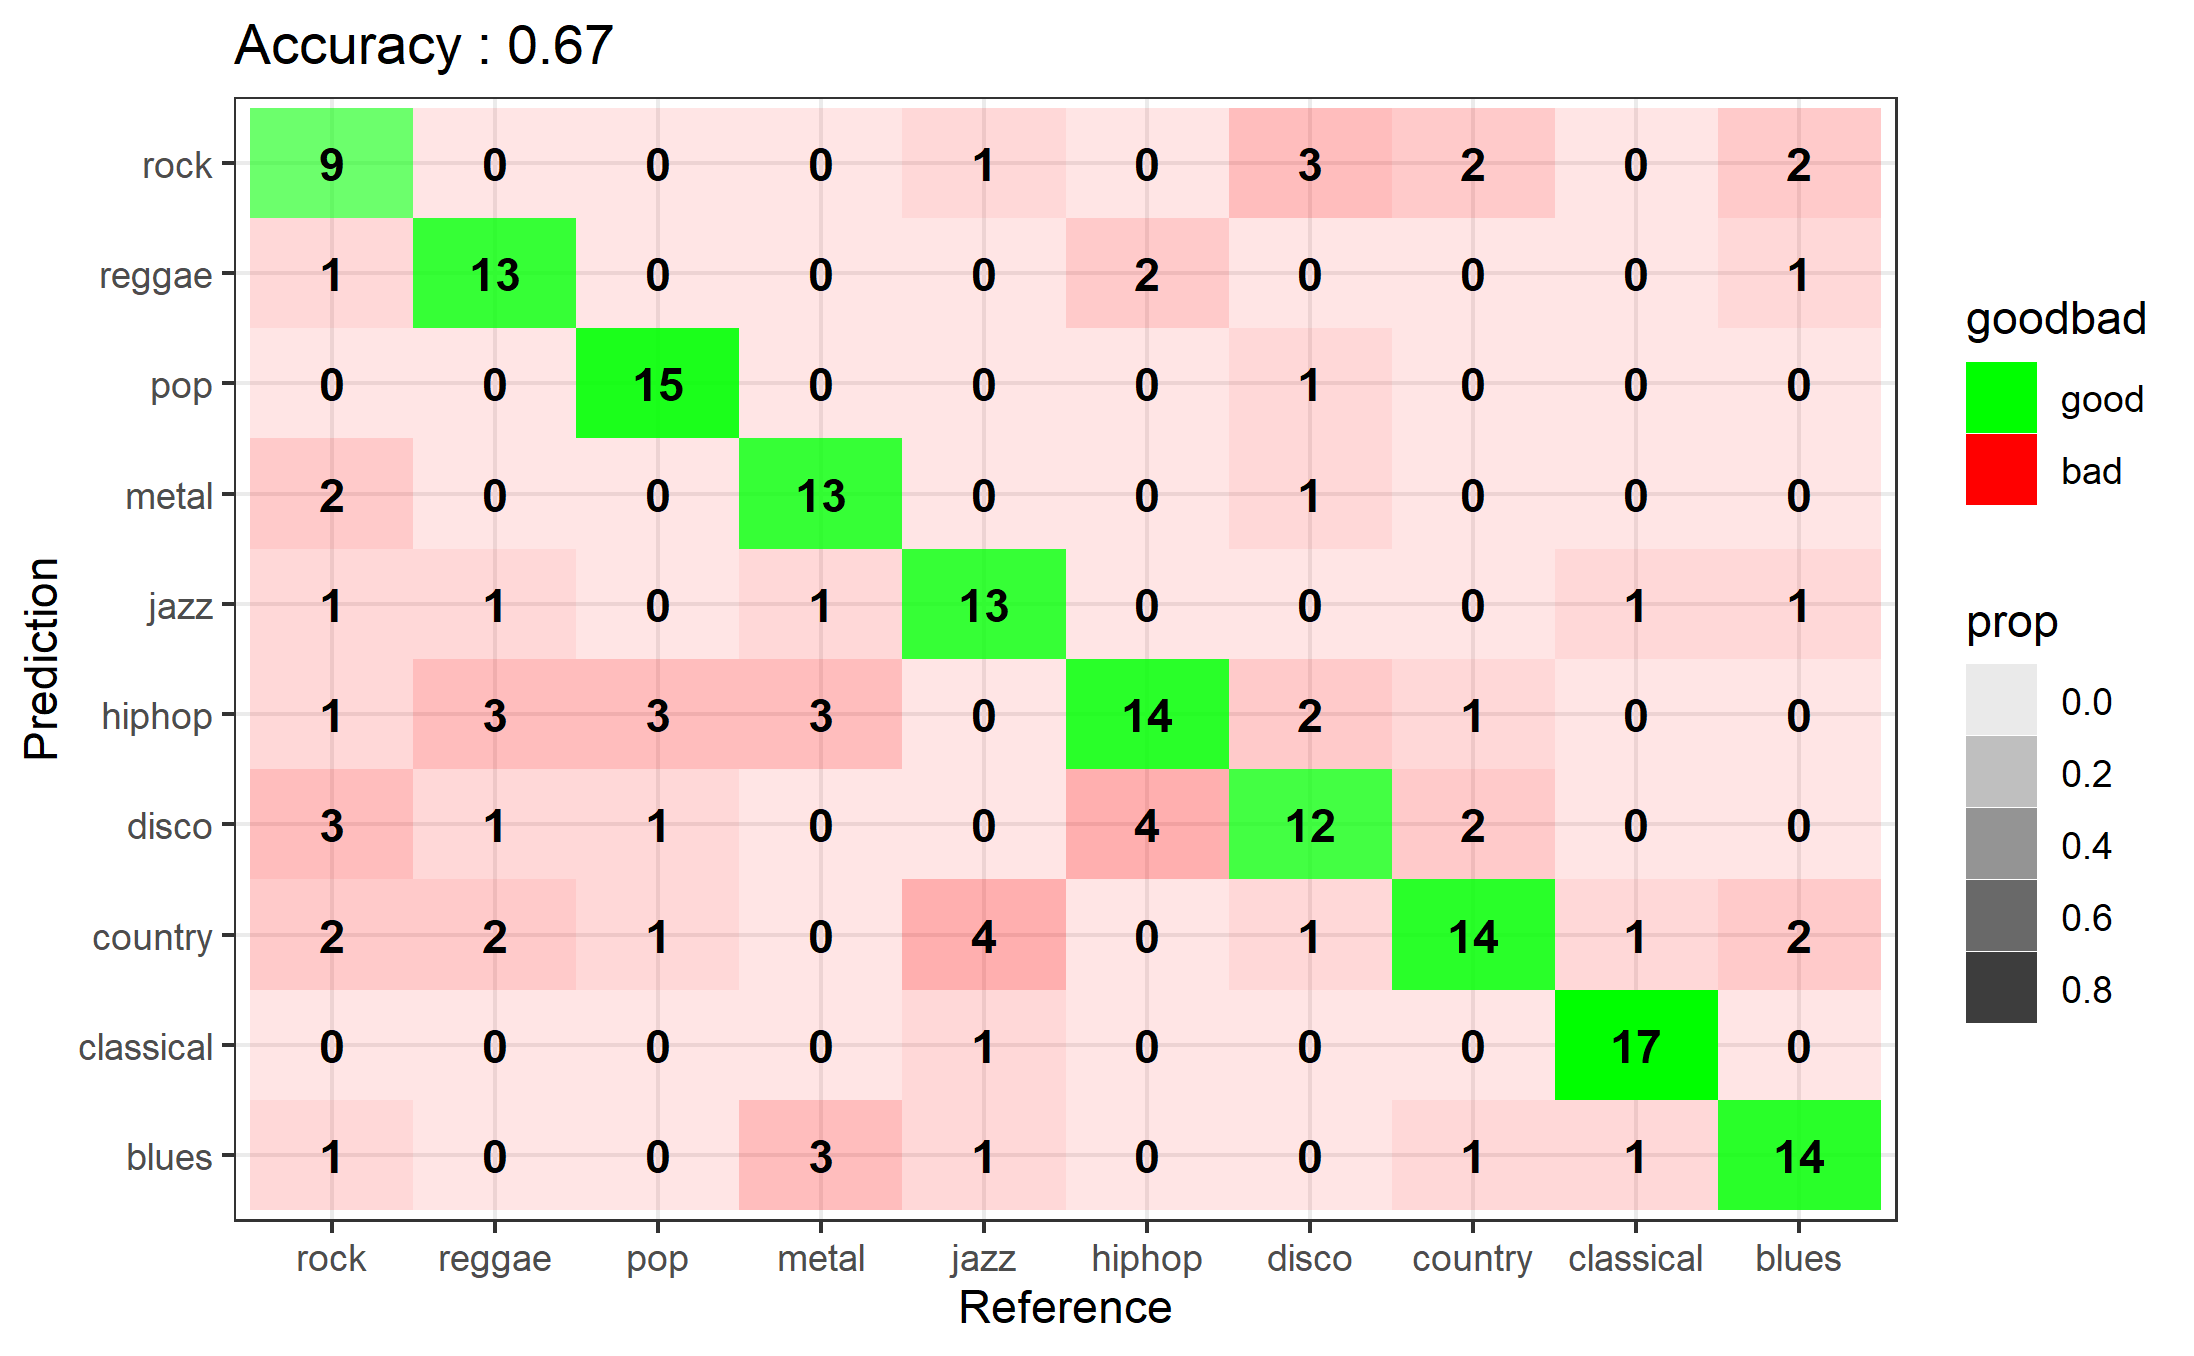
\includegraphics[width=0.8\textwidth]{confusionMatrix_svm.png}
\end{center}
\end{frame}

\begin{frame}{SVM(scaling)}
\begin{center}
    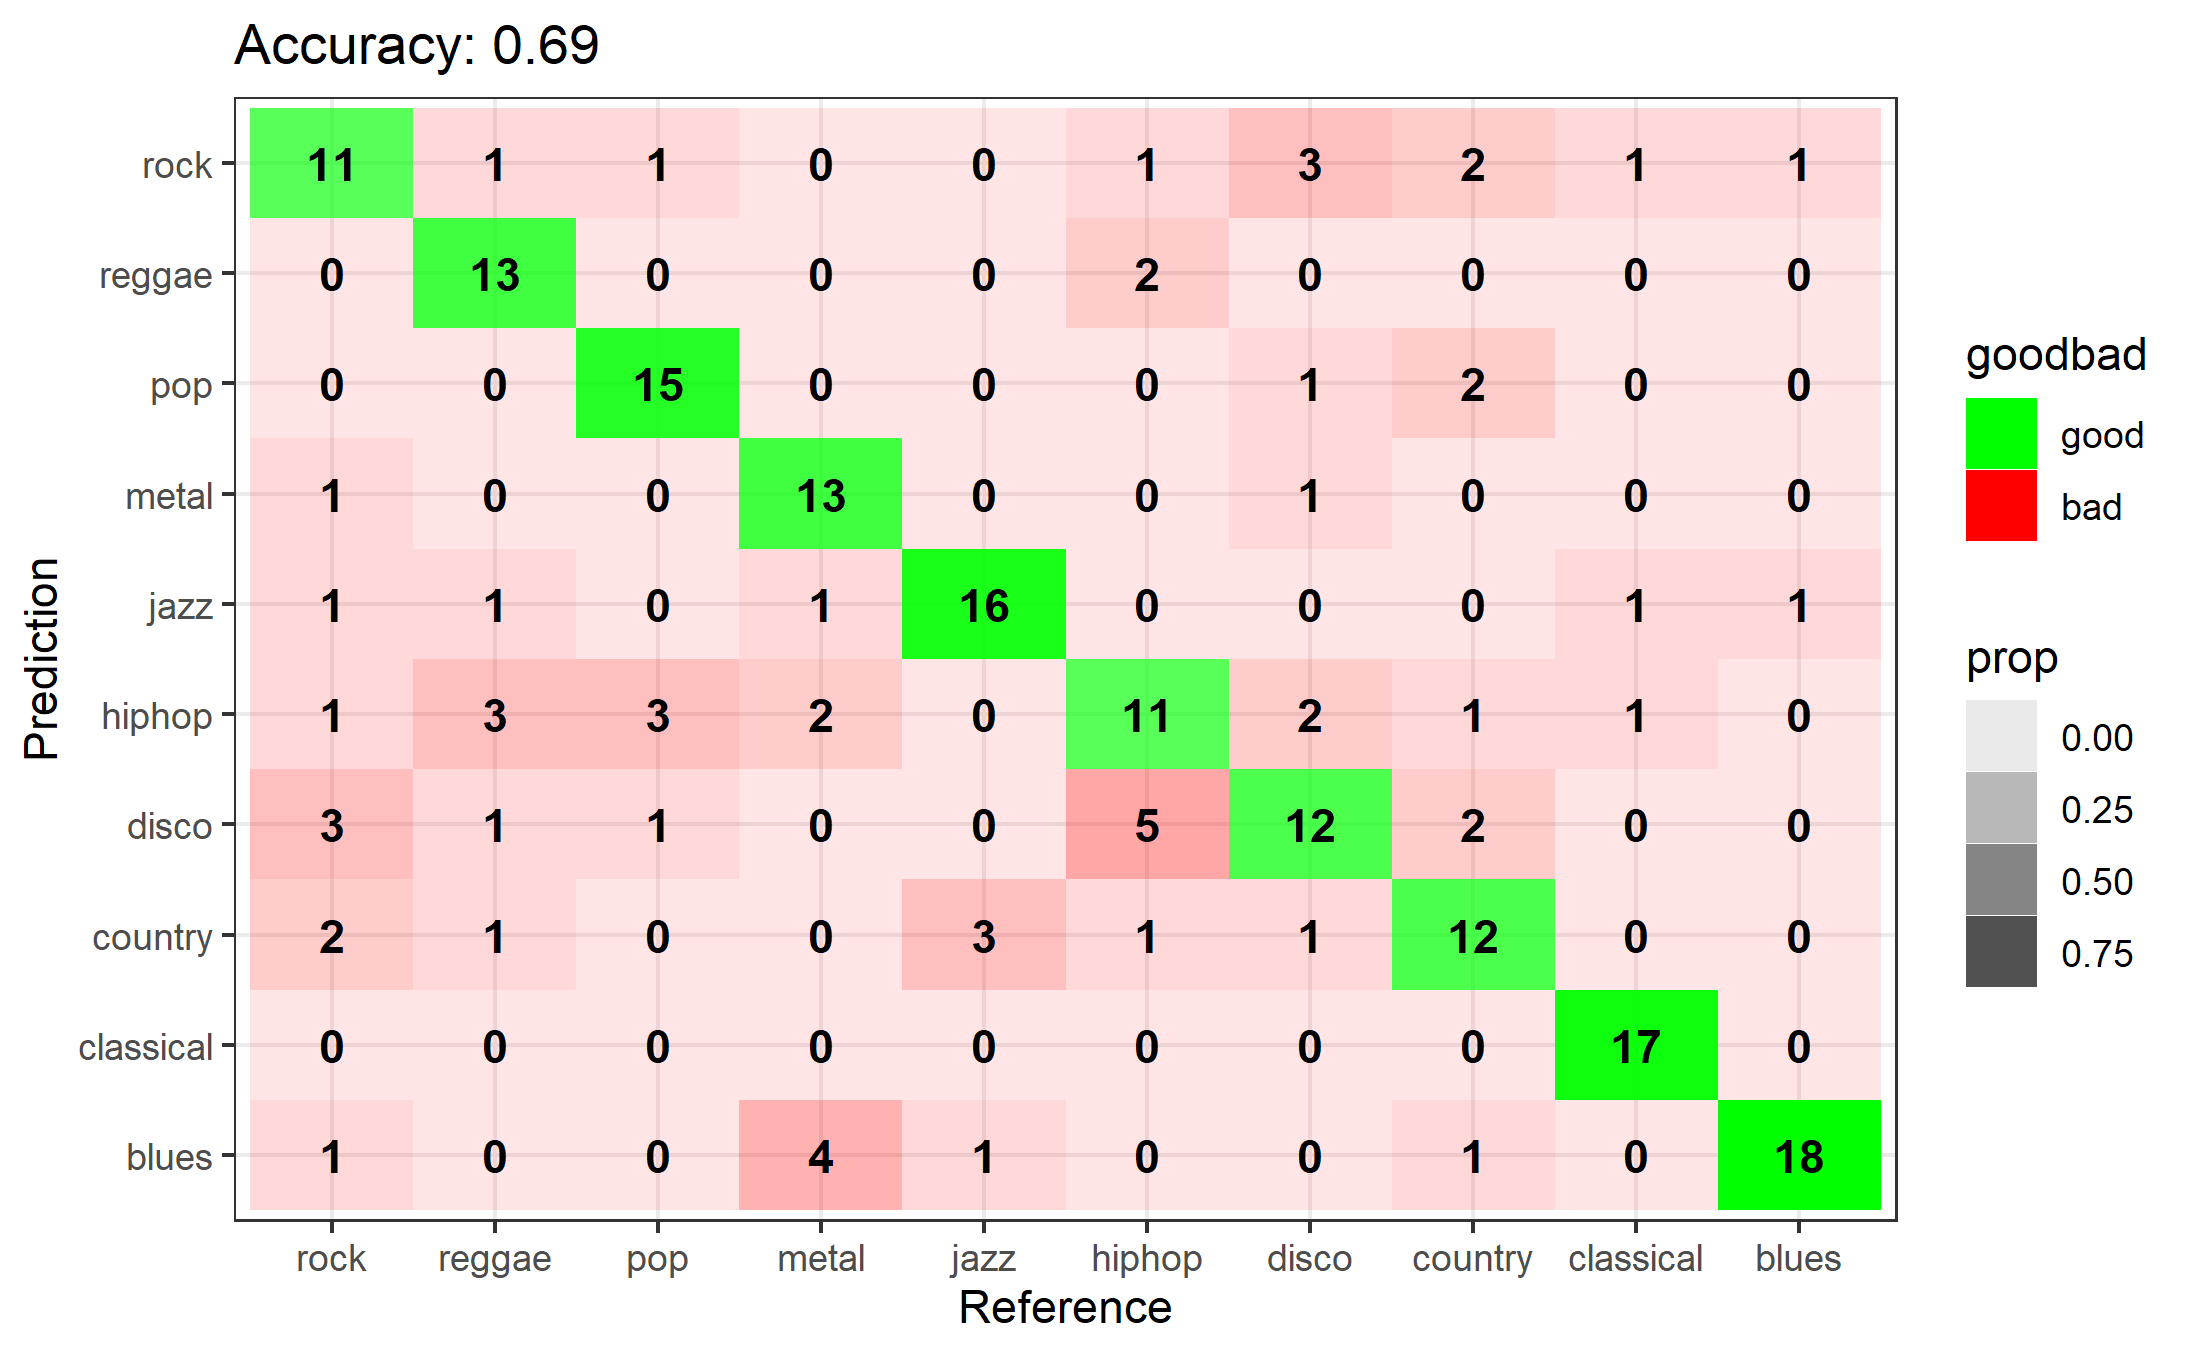
\includegraphics[width=0.8\textwidth]{confusionMatrix_svm_std.png}
\end{center}
\end{frame}

\begin{frame}{Random Forest}
\begin{center}
    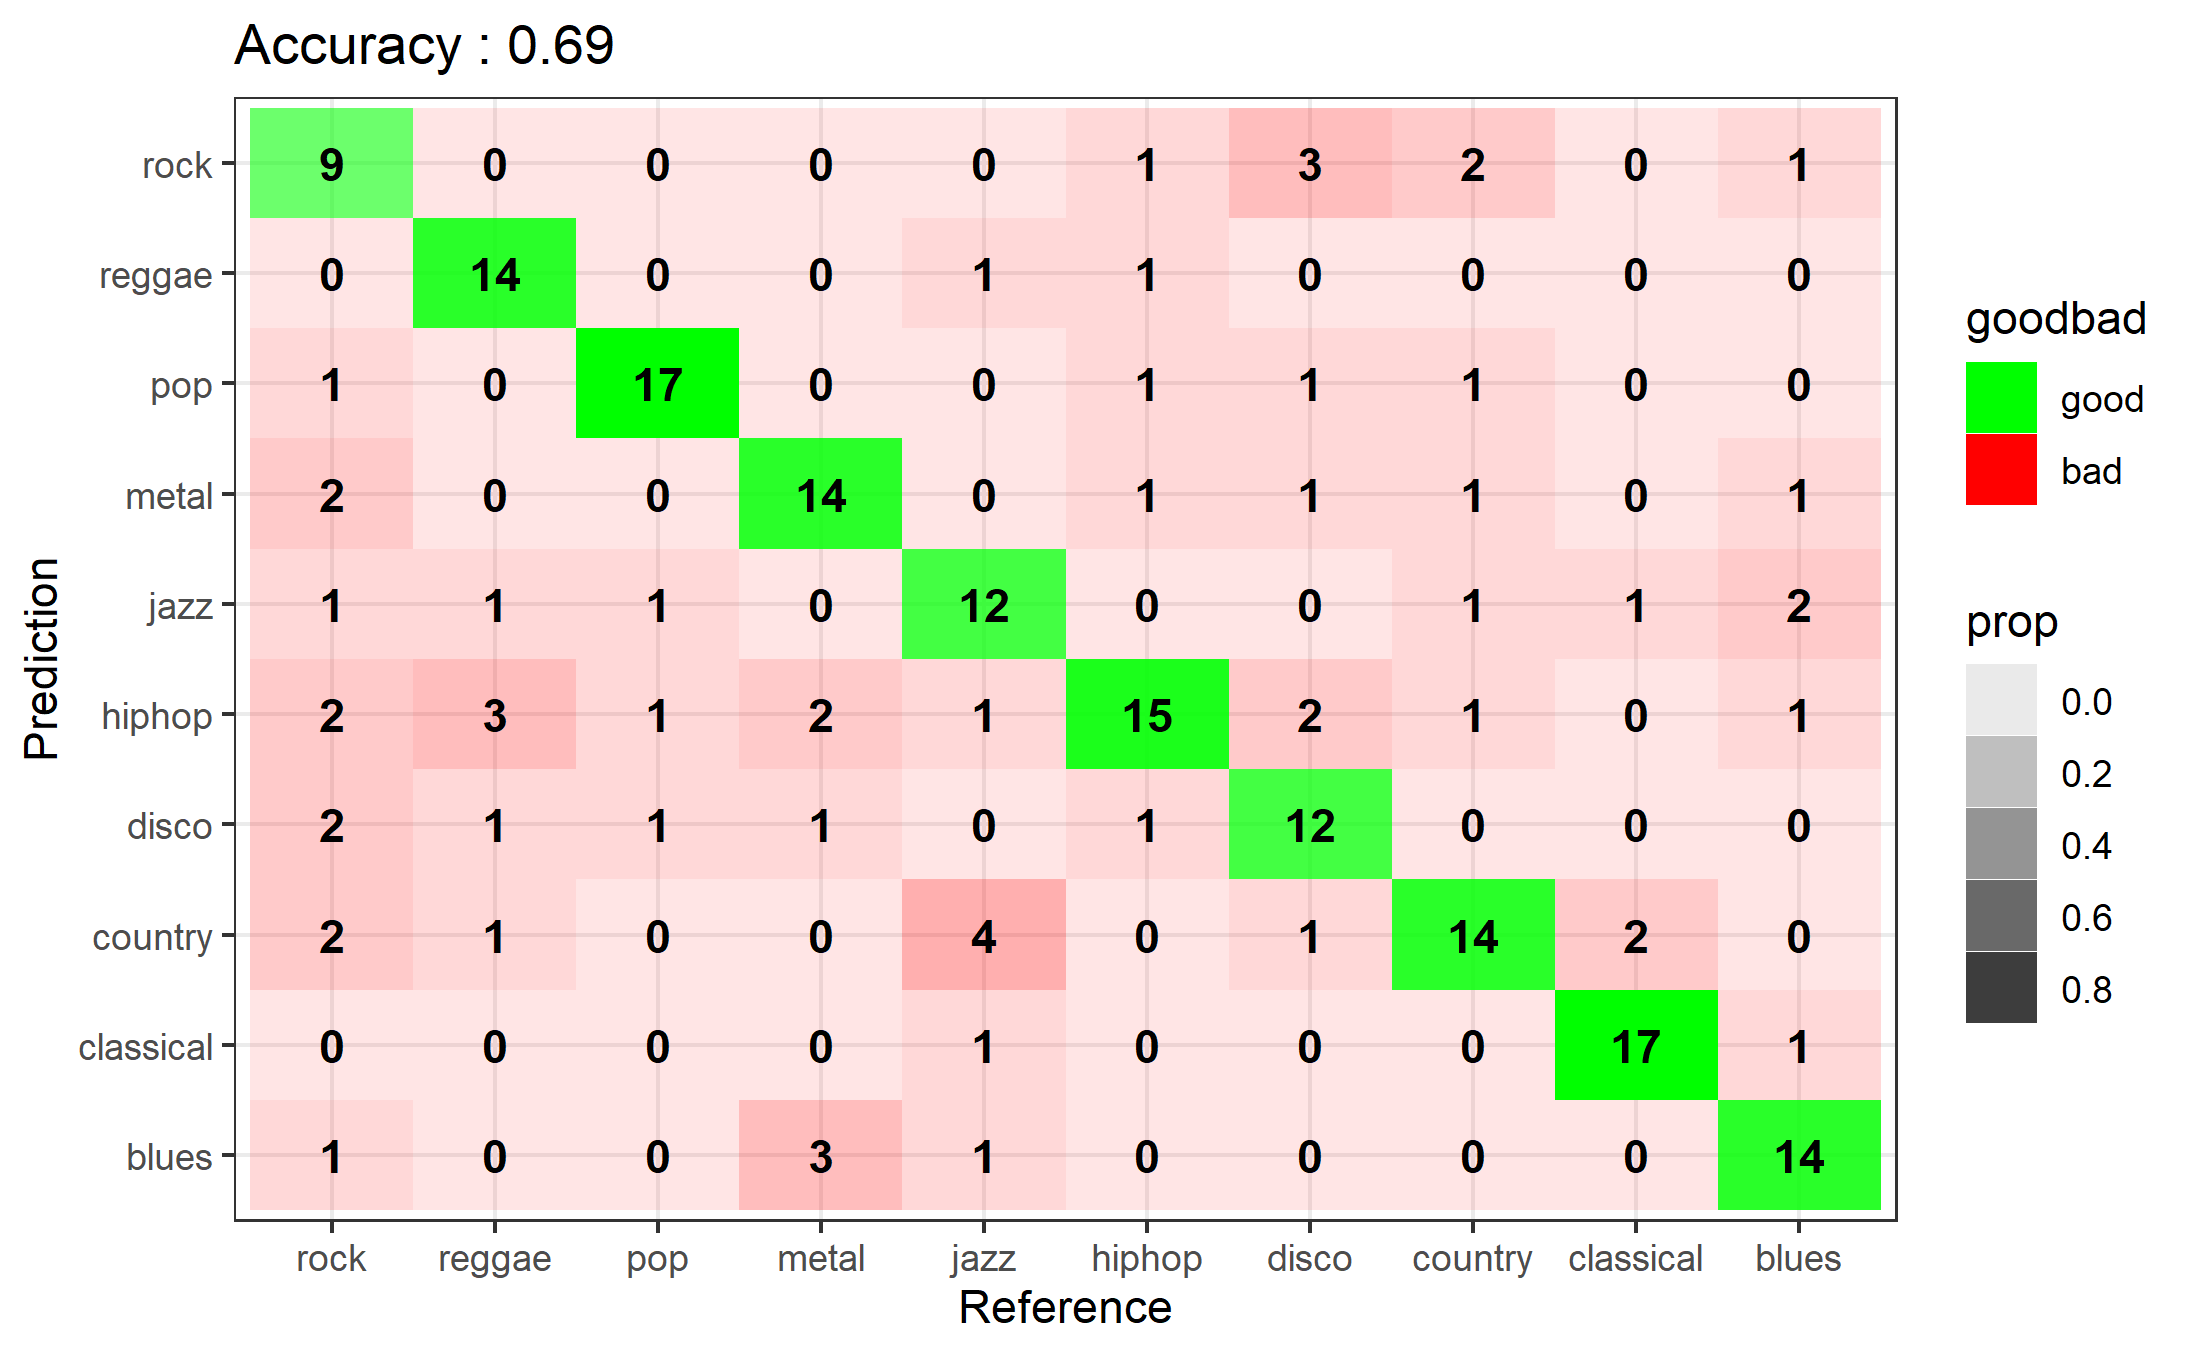
\includegraphics[width=0.8\textwidth]{confusionMatrix_randomforest.png}
\end{center}
\end{frame}

\begin{frame}{Random Forest(scaling)}
\begin{center}
    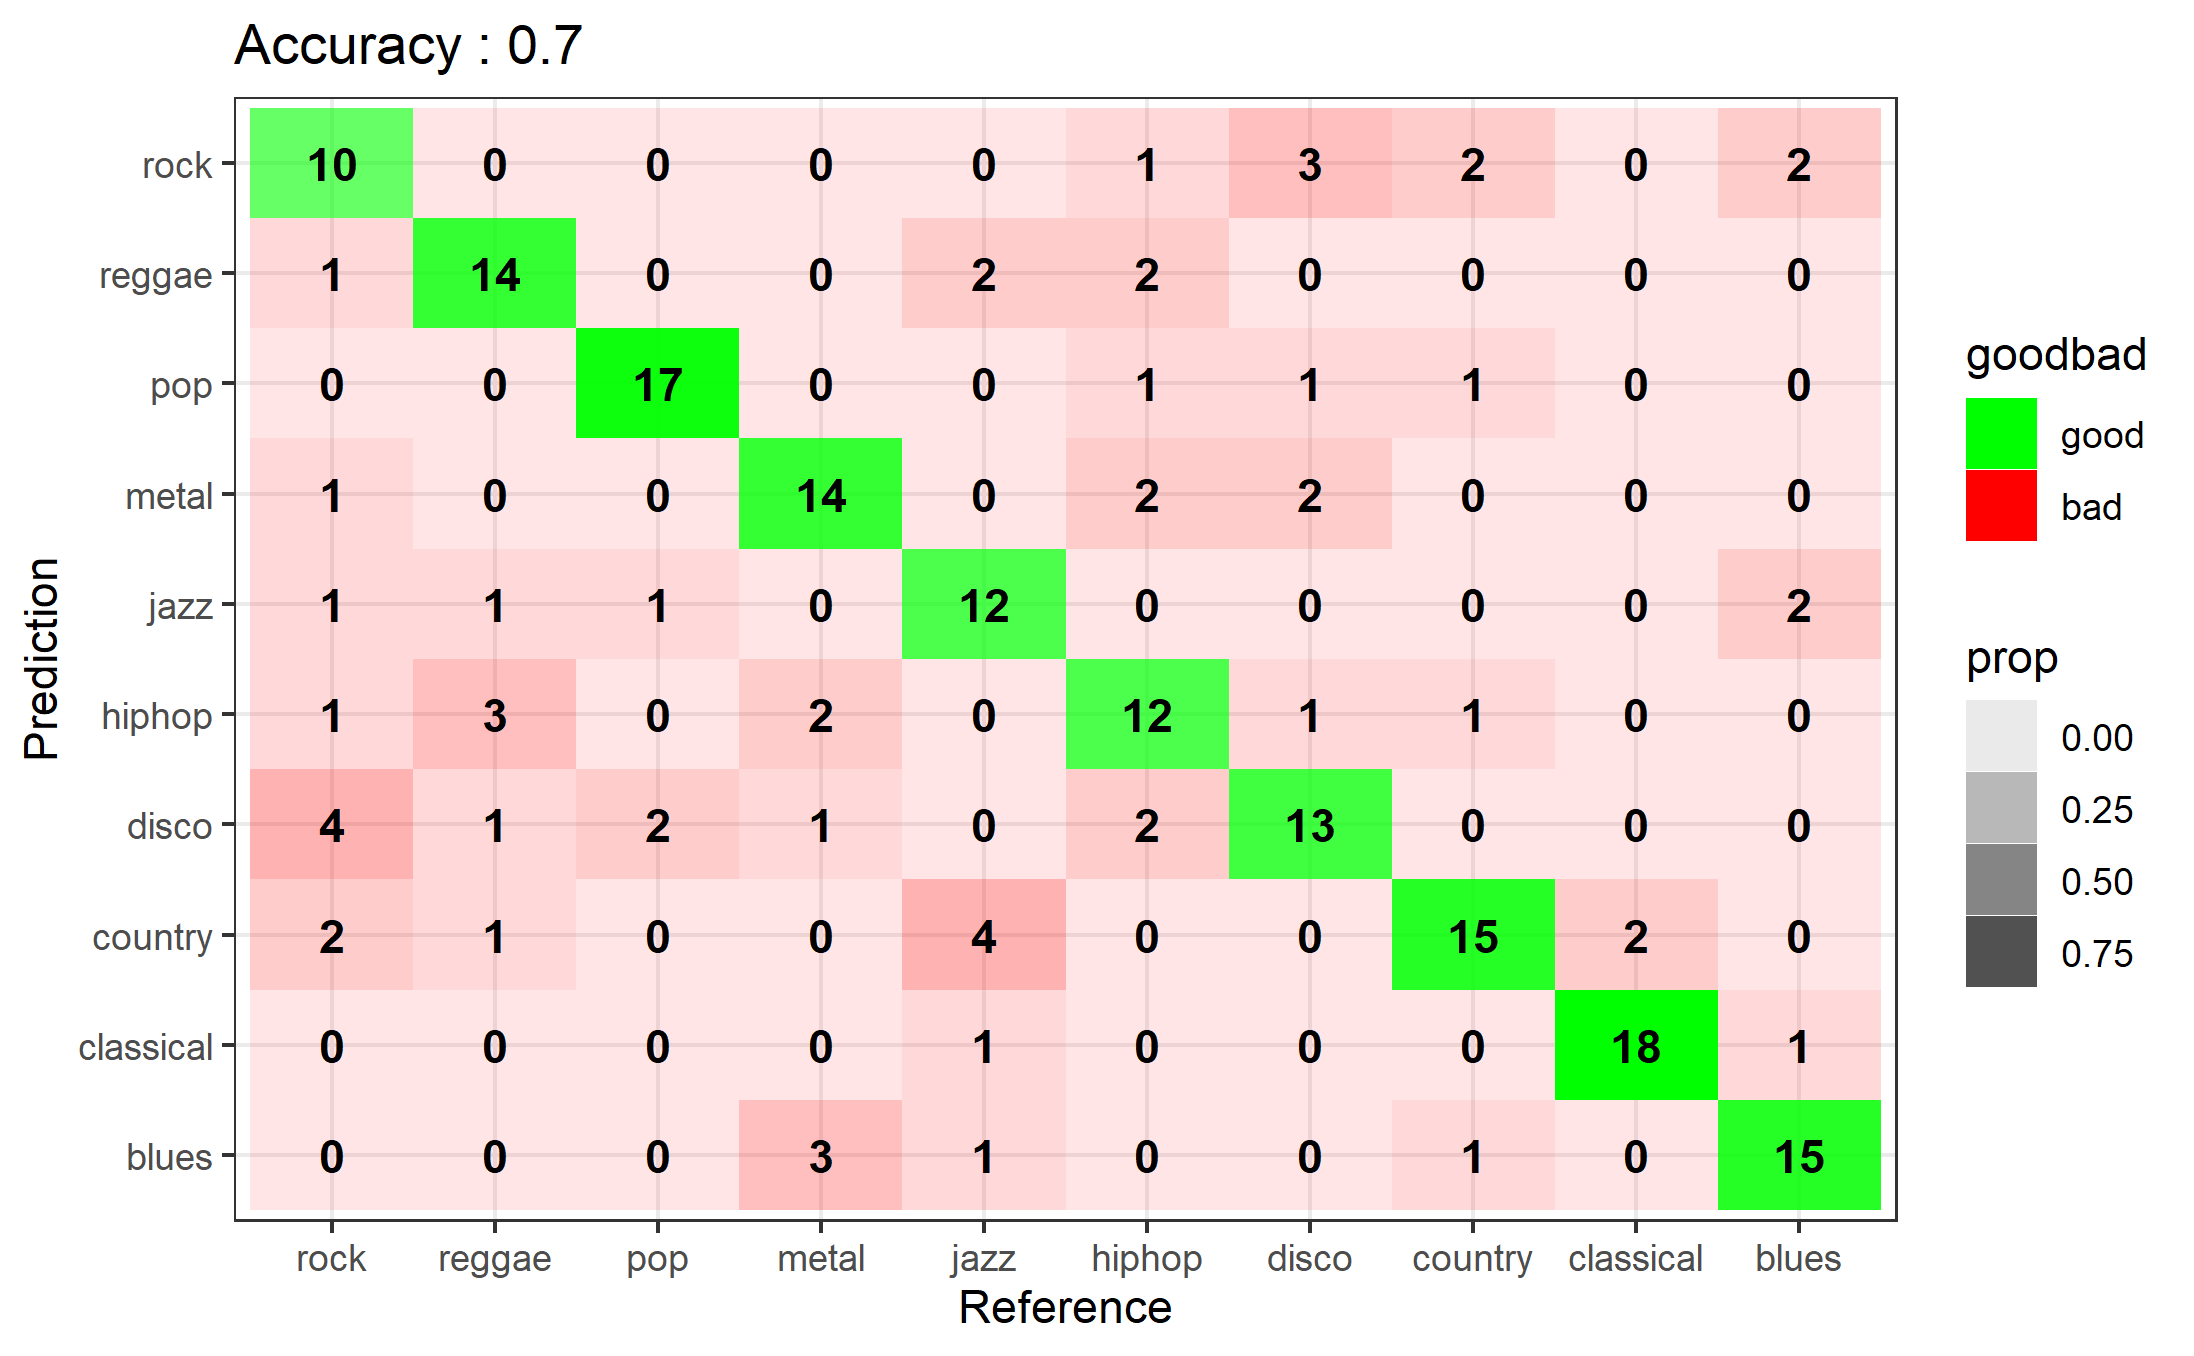
\includegraphics[width=0.8\textwidth]{confusionMatrix_randomforest_std.png}
\end{center}
\end{frame}

\section{Conclusion}
\begin{frame}{Conclusion}
\begin{itemize}
    \item Genre is classified.
    \item SVM and Random Forest are brilliant classifier.
\end{itemize}
\end{frame}

\section{Reference}
\begin{frame}{Reference}
\begin{itemize}
  \item (TextBook)Hastie, Tibshirani and Friedman (2009). The Elements of Statistical Learning: Data Mining, Inference and Prediction. 2nd Edition.
  \item (TextBook)Hardle and Simar (2015). Applied Multivariate Statistical Analysis, 4th Edition.
  \item (Paper)Chih-Wei Hsu, Chih-Chung Chang, and Chih-Jen Lin (2016). A Practical Guide to Support Vector Classification.
  \item  Meinard Muller, Stefan Balke (2015). Short-Time Fourier Transform and Chroma Features.
  \item (Website)\href{https://librosa.org/doc/latest/index.html}{Librosa} \item (Website)\href{https://www.britannica.com/story/whats-the-difference-between-tempo-and-rhythm}{Tempo vs Rhythm}
\end{itemize}
\end{frame}

\end{document}